\documentclass{article}

\usepackage{titlesec}
\usepackage{titling}
\usepackage[margin=0.7cm]{geometry}
\usepackage{float} 
\usepackage{graphicx}
\graphicspath{ {../img/} }
\usepackage{multirow}
\usepackage{booktabs}
\usepackage{hyperref}
\usepackage{xcolor}

\titleformat{\section}
{\Large\bfseries}
{}
{0em}
{}[\titlerule]

\titleformat{\subsection}
{\bfseries}
{}
{0em}
{}

\titleformat{\subsubsection}[runin]
{\bfseries}
{}
{0em}
{}

\titlespacing{\section}
{0em}{0em}{0.3em}
\titlespacing{\subsection}
{0em}{0em}{0em}
\titlespacing{\subsubsection}
{0em}{0em}{0.5em}

\setlength\intextsep{0mm}


\hypersetup{
  colorlinks=true,
  urlcolor=black!70!black
}

\begin{document}
\title{R\'esumm\'e}
\author{Carlos Herrera Valerio}



\begin{table}[ht]
\centering
	\begin{tabular}{p{5cm}p{6cm}p{6cm}}
	\multirow[t]{3}{*}[-2.3cm]{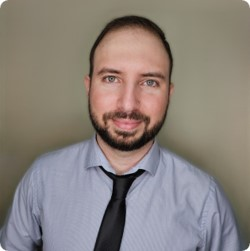
\includegraphics[width=0.16\textwidth]{profile_photo_1-1_rounded}} &
	\multicolumn{2}{c}{\huge\textbf{Carlos Herrera Valerio}} \\ &
	\begin{tabular}[c]{@{}l@{}}
		\\Electronic Engineer\\ 
		8+ years of experience\\ 
		Data Science\\ 
		Analog testing
	\end{tabular} &
		\multicolumn{1}{r}{
			\begin{tabular}[c]{@{}r@{}}
				\\(+506) 8894 4826\\ 
				\href{mailto:carlos.herrera.valerio@gmail.com}{carlos.herrera.valerio@gmail.com}\\ 
				\href{https://www.linkedin.com/in/carlosherreravalerio/}{linkedin.com/in/carlosherreravalerio}\\ 
				Heredia, Costa Rica
			\end{tabular}} \\
 &
\end{tabular}
\vspace{-12pt}
\end{table}

\section{About me}
\noindent
Experinced electronic engineer with over eight years in the semiconductor industry specializing in high-volume manufacturing, analog testing and electronic design validation of IOs. Seeking a career transition into data science and data analytics applied to manufacturing and problem-solving, looking for new work opportunities to align my job with my passion analyzing and understanding data to drive positive impact and innovation within the industry.

\section{Work Experience}
\subsection{Intel Costa Rica(2016 - Present day)}

\subsubsection{IO Design Validation of DDR Memory}
\subsubsection{2023 - Present day:}
To expand my background in IO IPs, I joined the IODV team where we utilize lab equipment to validate the correct functioning of DDR in Intel Xeon 6 products. To streamline our processes, we implemented a Python environment for automated measurement taking and data handling. I regularly write Python scripts and use JMP/JSL for automated data analysis. Additionally, we established a database to store our results.

\subsubsection{IO High Volume Manufacture}
\subsubsection{2022 - 2023:}
For Intel 5th Gen Xeon, I worked remotely as a Product Owner with Santa Clara’s High Speed IO team, enabling full test content within an aggressive schedule to prepare for Power On, frequently had to debug Python scripts and collaborate with designers and validation teams in Task Forces to implement the Gen5 Loopback test for UPI interfaces. As a result of the work done during this period, I was awarded for a remarkable, result-oriented effort.
\subsubsection{2019 - 2022:}
Working for Intel 3rd Gen Xeon I was able to contribute to the point where the product achieved quality goals, then led the team to fine tune health indicators using an analytic approach making sure defects were found as early as possible in the line while ensuring quality in the final product, working closely with designers and production teams, we reached DPM objective on time for the roadmap.
\subsubsection{2018:}
Early in my career, I was pulled from my daily work to support the Israeli team, which was struggling due to an unexpected headcount reduction and an impending deadline. A peer and I were sent to Israel to become more involved in solving yield issues with Intel's Client 10th Gen. My primarily contribution was in DoEs, integration, data analysis, and data review. By the end of this period, we successfully increased yield numbers to the desired goal, gaining valuable experience working abroad and collaborating with a different team to resolve a complex problem.

\section{Skills}
\noindent\textbf{Data Analysis:} Part of my daily work, I have analyzed vast amounts of data to identify opportunities for production improvements, pulling information from databases to create informative charts to present and communicate insights to other engineering teams to define an action plan.\\
\textbf{Team Work:} Throughout my six years of experience in High Volume Manufacturing activities, I have actively participated in task forces with multidisciplinary engineering teams to address silicon issues, debug test content, or reduce high fallout rates. I frequently analyze volume data to select DUTs for specific DoEs.\\
\textbf{Electronic Lab Equipment:} Use of lab equipment such as Scope, BER, DCPA, VNA, switches, and thermal controllers. Automating tasks utilizing SCPI commands and python libraries.\\
\textbf{Programming:} Experienced in writing and reading code following professional standats to contribute to modular development. Enthusiastic about using Machine Learning methods to solve problems.\\
\textbf{Programming languages/libraries:} Proficient in Python, JMP/JSL, R, PySpark, Docker, PyTorch, Pandas, Matplotlib, Numpy, SeaBorn, Matplotlib, Sklearn, Postgres, SQL, Tableau.\\
\textbf{Linux:} Comfortable working within Linux environment generating test content, automating, managing files and using \LaTeX .\\
\textbf{Languages:} Excellent written and verbal communication skills in English, and native in Spanish.

\section{Education}

\begin{table}[ht]
\centering
\begin{tabular}{lr}
	\begin{tabular}[c]{@{}l@{}}\textbf{FundaTec}\\ Data Science Program\end{tabular}                                                                                                                                                & \begin{tabular}[c]{@{}r@{}}\textbf{Cartago, Costa Rica}\\ Graduated September 2024\end{tabular}     \\
		\begin{tabular}[c]{@{}l@{}}\textbf{Costa Rica Institute of Tecnology(TEC)}\\ Licentiate Electronic Engineering\end{tabular}                                                                                                     & \begin{tabular}[c]{@{}r@{}}\textbf{Cartago, Costa Rica}\\ Graduated June 2016\end{tabular}     \\
			\begin{tabular}[c]{@{}l@{}}\textbf{University Center Miravalles}\\ Professional Development Program (PDP)\\ Reinforcement of soft skills, integrity, communication, emotional intelligence and abilities for life.\end{tabular} & \begin{tabular}[c]{@{}r@{}}\textbf{San Jose, Costa Rica}\\ Graduated December 2015\end{tabular}
\end{tabular}
\end{table}

\section{References}
\begin{flushleft}
Didier Chacón | Manager from 2019 to 2023\\
Enrique Con | Product Owner and peer\\
%Sheryl Johnes | US peer \\
%Gustavo Aguilar | Mentor \\

\end{flushleft}

\end{document}
